% Možné jazyky práce: czech, english
% Možné typy práce: BP (bakalářská), DP (diplomová)
\documentclass[czech,DP]{thesiskiv}

\author{Bc. David Pivovar}
\declarationmale

% Název práce
\title{Detekce vybraných aktivit diabetického pacienta 1.~typu}

% 
% Texty abstraktů (anglicky, česky)
%
\abstracttexten{The text of the abstract (in English). It contains the English translation of the thesis title and a short description of the thesis.}

\abstracttextcz{Text abstraktu (česky). Obsahuje krátkou anotaci (cca 10 řádek) v češtině. Budete ji potřebovat i při vyplňování údajů o bakalářské práci ve STAGu. Český i anglický abstrakt by měly být na stejné stránce a měly by si obsahem co možná nejvíce odpovídat (samozřejmě není možný doslovný překlad!).
}

% Na titulní stranu a do textu prohlášení se automaticky vkládá 
% aktuální rok, resp. datum. Můžete je změnit:
%\titlepageyear{2016}
%\declarationdate{1. března 2016}

% Ve zvláštních případech je možné ovlivnit i ostatní texty:
%
%\university{Západočeská univerzita v Plzni}
%\faculty{Fakulta aplikovaných věd}
%\department{Katedra informatiky a výpočetní techniky}
%\subject{Bakalářská práce}
%\titlepagetown{Plzeň}
%\declarationtown{Plzni}

%%%%%%%%%%%%%%%%%%%%%%%%%%%%%%%%%%%%%%%%%%%%%%%%%%%%%%%%%%
%
% DODATEČNÉ BALÍČKY PRO SAZBU
% Jejich užívání či neužívání záleží na libovůli autora 
% práce
%
%%%%%%%%%%%%%%%%%%%%%%%%%%%%%%%%%%%%%%%%%%%%%%%%%%%%%%%%%%

% Zařadit literaturu do obsahu
\usepackage[nottoc,notlot,notlof]{tocbibind}

% Umožňuje vkládání obrázků
\usepackage[pdftex]{graphicx}
\usepackage{float}
\usepackage{rotating}

% Odkazy v PDF jsou aktivní; navíc se automaticky vkládá
% balíček 'url', který umožňuje např. dělení slov
% uvnitř URL
\usepackage[pdftex,]{hyperref}
\hypersetup{colorlinks=true,
  unicode=true,
  linkcolor=black,
  citecolor=black,
  urlcolor=black,
  bookmarksopen=true}

% Při používání citačního stylu csplainnatkiv
% (odvozen z csplainnat, http://repo.or.cz/w/csplainnat.git)
% lze snadno modifikovat vzhled citací v textu
\usepackage[numbers,sort&compress]{natbib}
\usepackage{amsmath}

%%%%%%%%%%%%%%%%%%%%%%%%%%%%%%%%%%%%%%%%%%%%%%%%%%%%%%%%%%
%
% VLASTNÍ TEXT PRÁCE
%
%%%%%%%%%%%%%%%%%%%%%%%%%%%%%%%%%%%%%%%%%%%%%%%%%%%%%%%%%%
\begin{document}
%
\maketitle
\tableofcontents
\parskip=6pt
\chapter{Úvod}

Diabetes mellitus je rozšířené chronické metabolické onemocnění. Vyznačuje se zvýšenou koncentrací cukru v krvi (glykémie), která vniká z nedostatku inzulinu nebo rezistencí vůči jeho působení. Hlavní součástí léčby je monitorace koncentrace glukózy a podávání inzulinu. V dnešní době je možné sledovat vývoj glykémie díky sytémům kontinuální monitorace glukózy (CGMS) a kontinuálnímu dávkování inzulinu díky inzulinovým pumpám. Integrace těchto dvou systémů umožňuje autonomní řízení dávkování inzulinu v závislosti na aktuální koncentraci glukózy.

Koncentraci glukózy v krvi ovlivňuje mnoho faktorů. Dva nejvýznamnější faktory jsou příjem karbohydrátů a fyzická aktivita. Tyto aktivity je třeba kompenzovat zvýšením či snížením množství podávaného inzulinu. Aktuálně je do CGMS zadává pacient a dávku inzulinu upravuje také on. Monitorace těchto aktivit slouží pro správné nastavení léčby diabetologem. Jejich včasná detekce by umožnila přesnější monitoraci vývoje glykémie a lepší řízení autonomních systémů s minimálním zásahem pacienta.

V mé práci se budu zabývat možnostmi detekce příjmu kabohydrátů a fyzické aktivity z dat senzoru CGMS. Následně tyto metody implementuji do aplikace SmartCGMS vyvíjené na katedře informatiky a výpočetní techniky na ZČU.
\chapter{Diabetes mellitus}

Diabetes mellitus je chronické metabolické onemocnění. Vyznačuje se zvýšenou hladinou cukru v krvi, která se nazývá hyperglykémie. V normálu je hladina glykémie (koncentrace glukózy v krvi) mezi 3,8 a 5,6 mmol/l. Po jídle může glykémie stoupnout, neměla by však přesáhnout 7,8 mmol/l. O diabetes se jedná pokud jsou hodnoty vyšší než 11,1 mmol/l.

Hyperglykémie vzniká z nedostatku inzulinu nebo rezistencí buněk vůči jeho působení. Inzulin je hormon, který se tvoří v beta buňkách Langerhansových ostrůvků ve tkáni slinivky břišní. Tento hormon slouží k transportu glukózy z krve do tkáně, kde je využita k tvorbě energie nebo se zde ukládá ve formě glykogenu (v játrech) a tuků. Snižuje tak hladinu cukru v krevním řečišti. Pokud je hladina cukru nízká, produkce inzulinu se okamžitě zastaví  a hormony glukagon a adrenalin uvolní glukózu ze zásobních zdrojů pro zajištění fungování důležitých orgánů, především mozku, nervů a svalů.

Nedostatek inzulinu vede k nedostatečné utilizaci glukózy, která se hromadí v krvi. Dochází k poruše tvorby bílkovin, zvýšené tvorbě ketolátek, které se hromadí a způsobují překyselení organismu, a celkovému metabolickému rozvratu. Při hladině glykémie vyšší než 10-12 mmol/l začnou ledviny uvolňovat glukózu do moči spolu s dalšími látkami a vodou. To vše vyvolává dehydrataci, nevolnost, pokles krevního tlaku, poruchy vědomí.

Dlouhodobě přetrvávající hyperglykémie vede k poškození orgánů, především cév, nervového systému, ledvin a očí. Poškozením velkých cév může dojít k srdečnímu infarktu, mozkové příhodě nebo uzavření tepen v oblasti dolních končetin (ischemická choroba dolních končetin). U diabetických pacientů mají tato onemocnění komplikovanější průběh a vyšší úmrtnost. Nervové poškození je označováno jako diabetická neuropatie. Nejčastěji se objevuje v oblasti dolních končetin. končetina ztrácí citlivost, kůže vysychá a tvoří se defekt do kterého se snadno dostane infekce. Pokud není včas léčen, rozvíjí se syndrom diabetické nohy, který může vést k amputaci končetiny. poškození ledvin může vést k dialýze až k transplantaci ledvin. Poškození očí je příčinou vzniku šedého zákalu.

Bez léčby inzulinem může toto onemocnění vést k smrti. \cite{Diabetes.Psottova,Wikiskripta,cukrovka.cz,Diabetes.TaiN}


\section{Dělení diabetu}

Diabetes se dělí do čtyř základních skupin: diabetes 1. typu, diabetes 2. typu, gestační (těhotenský) diabetes, jiné specifické typy diabetu.

Diabetes mellitus 1. typu je autoimunitní onemocnění kdy vlastní imunitní systém zničí beta buňky Langerhansových ostrůvků produkující inzulin. Při zničení 75-85\% je absolutní nedostatek inzulinu a objevují se zvýšené hodnoty glykémie. Diabetes 1. typu se nejčastěji projeví již v dětském věku, ale může dlouho probíhat v latentní formě a projevit se až v pozdějším věku (LADA - latentní autoimunitní diabetes u dospělých). Že se jedná o LADA a ne diabetes 2. typu se určí detekcí autoprotilátek, které vznikají při poškozování beta buněk. Nemoc se projevuje častým močením, hubnutím a celkovou slabostí. Příčina vzniku diabetu 1. typu není známá a vlohy jsou často dědičné. Protože příčina vzniku není známa, není žádná účinná prevence.

Diabetes mellitus 2. typu je metabolickou poruchou kdy jsou buňky rezistentní vůči vlastnímu inzulinu, tj. buňky nejsou schopny vychytat inzulin v krevním oběhu, který by použili ke zpracování glukózy a úpravě hladiny glykémie. V počátcích beta buňky slinivky břišní reagují zvýšenou produkcí inzulinu (bezpříznaková inzulinová rezistence). Postupem času ale nejsou schopny dodávat potřebné množství inzulinu, nastává relativní nedostatek inzulinu a vzniká prediabetes a diabetes 2. typu. Příznaky jsou únava, žízeň, časté močení, pocit hladovění, hubnutí, infekce, špatné hojení a zhoršení zraku. Diabetes mellitus 2. typu vzniká v dospělosti na základě genetických předpokladů (inzulinová rezistence, nízká produkce inzulinu), rizikových faktorů a špatného životního stylu. Mezi ty patří nedostatek pohybu, nezdravá strava, nadváha a obezita (90\% diabetiků 2. typu trpí nadváhou nebo je obézních), kouření, vysoká hladina cholesterolu a vysoký krevní tlak (hypertenze).

Gestační diabetes se objevuje v druhé polovině těhotenství a končí po porodu. Postihuje 17\% těhotných žen, které k ní mají vrozenou dispozici. Neléčený diabetes má negativní dopad na vývoj plodu, který se musí vyrovnat se zvýšeným přísunem glukózy. Plod, který má produkci inzulinu v pořádku, pak výrazně rychleji roste. To může vést k předčasnému porodu, vrozeným vývojovým vadám, dechovým obtížím, poruchám srdečního rytmu, poruchám vývoje mozku, sklon k obezitě a rozvoje diabetu 2. typu.

Jiné specifické typy diabetu se označují jako sekundární diabetes, protože k rozvoji diabetu dochází v důsledku jiného onemocnění (např. zánět slinivky břišní).

V České republice je evidováno více než 900 000 pacientů s diabetem. 92\% připadá na diabetes 2. typu, 7\% na diabetes 1. typu. Ročně přibude 60 tisíc nových diabetických pacientů a 22 tisíc umírá. Náklady na léčbu jednoho pacienta jsou okolo 26 000 Kč za rok. Ročně se tak vydá na léčbu diabetu 23 miliard Kč. \cite{Diabetes.Psottova,cukrovka.cz,Diabetes.TaiN}

Celosvětově je Světovou zdravotnickou organizací evidováno více než 422 milionů lidí s diabetem \cite{WHO}.

V této práci se budu zabývat detekcí karbohydrátů a fyzické aktivity u pacientů s diabetem 1. typu.


\section{Léčba}

Diabetes mellitus 1. typu je onemocnění z nedostatečné produkce inzulinu slinivkou a vždy se léčí podáváním inzulinu. Způsob léčby a množství podávaného inzulinu je rozebráno v kapitole \ref{ch:inzulin}, způsoby podání v kapitole \ref{ch:pumpa}. Další možností pro pacienty diabetu 1. typu je transplantace slinivky břišní nebo transplantace samotných Langerhansových ostrůvků.

Při léčbě inzulinem se musí dbát na to, aby nenastala hypoglykémie. Hypoglykémie je stav, kdy dochází k poklesu cukr v krvi pod 3,9 mmol/l. Příznaky jsou pocení, třes, bušení srdce, slabost. Při těžké hypoglykémii dochází k poruchám vědomí a je nutná pomoc jiné osoby. Může nastat i smrt. K hypoglykémii často dochází při podání příliš velké dávky inzulinu snahou regulovat hladinu glukózy co nejvíce k normálním hodnotám. Z toho důvodu by pacient měl mít u sebe menší množství rychlých cukrů pro doplnění při zpozorování prvních příznaků.

Zvýšené riziko těžké hypoglykémie je při poruše tvorby adrenalinu v nadledvinách. Adrenalin se uvolňuje při nízké hladině cukru v krvi a je zodpovědný za příznaky hypoglykémie. Pacient pak není schopen rozpoznat rozvíjející se hypoglykémii. Tato porucha se označuje jako syndrom porušeného vnímání hypoglykémie.

Diabetes mellitus 2. typu se nejprve léčí úpravou životosprávy a kombinace perorálně podávaných antidiabetik (léky zvyšující produkci inzulinu a/nebo citlivost buněk k inzulinu). Pokud se těmito prostředky nedaří regulovat hladina cukr v krvi, přidá se k podávaným antidiabetikám léčba inzulinem.

Společnými režimovými opatřeními pro oba typy diabetu je monitorace glukózy (viz kapitola \ref{ch:monitorace}), dieta a fyzická aktivita.

Glykemie je závislá na jídle, druhu a frekvenci stravy, proto patří dieta mezi základní opatření při léčbě cukrovky. Pacient by měl znát složení jídla, především množství zkonzumovaných sacharidů. Strava by měla být vyvážená a v pravidelných intervalech.

Pohyb je důležitý protože napomáhá účinnosti inzulinu. Při pohybu se také využije více glukózy na energii, je prevencí proti nadváze a obezitě a celkově prospívá organismu. Fyzická aktivita tak výrazně snižuje koncentraci glukózy v krvi. Ideální hodnota glykémie před fyzickou aktivitou je 6-7 mmol/l. Při nižších hodnotách hrozí riziko hypoglykémie. Naopak při hodnotách >15 mmol/l se postupuje jako při hyperglykémii.. Před aktivitou je vhodné snížit množství inzulinu.

Cílem léčby je udržení doporučených hodnot vybraných ukazatelů popsaných v tabulce \ref{tab:ukazatele}. V závorkách jsou uvedeny přijatelné hodnoty rizikových pacientů. Pakliže se pacientovi dlouhodobě daří udržovat tyto doporučené hodnoty, sníží riziko komplikací spojených s diabetem.
\cite{Diabetes.Psottova,cukrovka.cz}

\begin{table}[H]
\caption{Doporučené hodnoty vybraných ukazatelů}
\label{tab:ukazatele}
\centering
\begin{tabular}{|c|c|}
\hline 
\textbf{Ukazatel} & \textbf{Doporu\v{c}ené hodnoty}\tabularnewline
\hline 
\hline 
glykovaný hemoglobin & pod 45 (60) mmol/l\\ \hline 
glykémie naměřená před jídlem & 4-6 (pod 8) mmol/l\\ \hline 
glykémie naměřená po jídlem & 5-7,5 (pod 9) mmol/l\\ \hline 
krevní tlak & pod 130/80 (pod 140/90) mmHg\\ \hline 
celkový cholesterol & pod 4,5 mmol/l\\ \hline 
LDL-cholesterol & pod 2,5 mmol/l\\ \hline 
HDL-cholesterol (muži/ženy) & nad 1/1,2 mmol/l\\ \hline 
Celková denní dávka inzulinu & pod 0,6 j./kg\\
\hline 
\end{tabular}
\textit{Zdroj: www.cukrovka.cz}
\end{table}


\subsection{Inzulinové režimy}
\label{ch:inzulin}

Schéma léčby inzulinem se volí individuálně. Cílem je korigovat deficit inzulinu a co nejpřesněji simulovat fyziologickou sejreci inzulinu. Pro každého diabetického pacienta je toto jiné z důvodu vlastního metabolismu, životního stylu a aktivit.

Zpravidla dělíme dávkování inzulinu na bazální hladinu inzulinu a bolusy. Bazální hladina inzulinu zajišťuje správnou hladinu glykémie mezi 5-9 mmol/l během noci. Dávka podaného inzulinu musí být nastavena tak, aby nedošlo k hypoglykémii. Inzulin se podává buď v jedné dávce na noc, nebo ve dvou menších dávkách ráno a večer. Účinnost podání bazálního inzulinu v jedné dávce večer je vidět na obrázku \ref{fig:inzulin} modře. Používají se středně nebo dlouho působící inzuliny.

Před jídlem se podává rychle působící prandiální inzulin, bolus. Podává se 30 minut před jídlem a vrchol působení je mezi 1-2 hodinami. Jeho množství by mělo odpovídat velikosti jídla. Pro výpočet množství sacharidů pokrytých 1 jednotkou inzulinu aplikovaného před jídlem vydělíme číslo 500 celkovou denní dávkou inzulinu. Pro výpočet bolusu pak vydělíme množství přijatých sacharidů vypočtenou hodnotou. Podání bolusu před jídlem je znázorněno na obrázku \ref{fig:inzulin} červeně.

Bolus se může aplikovat i pokud se naměří zvýšená hladina glykémie (opravný bolus). Odhad poklesu glykémie po podání jedné jednotky inzulinu se vypočte 83 děleno celkovou denní dávkou inzulinu.
\cite{cukrovka.cz,Diabetes.Rybka,Inzulinove.rezimy}

\begin{figure}[H]
\caption{Působení inzulinu}
\label{fig:inzulin}
\centering
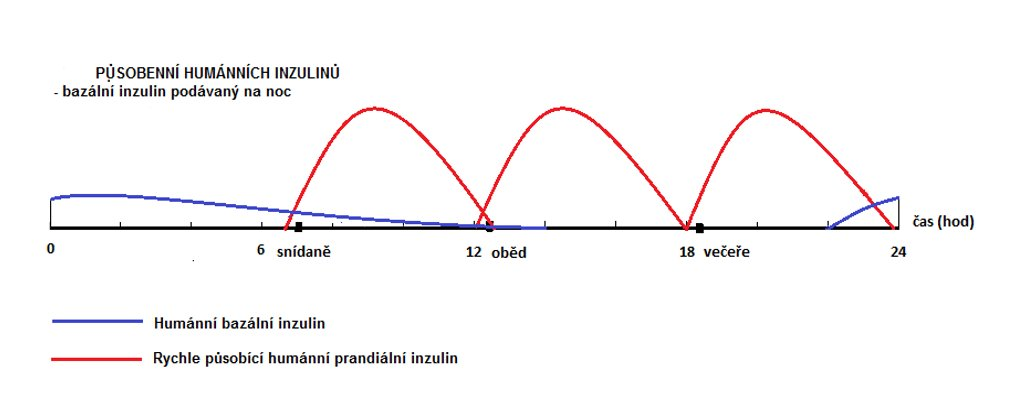
\includegraphics[width=1\textwidth]{img/pusobeni-humannich-inzulinu.jpg}
\textit{Zdroj: www.cukrovka.cz}
\end{figure}

Další možností je postupné dávkování inzulinu v malých dávkách během celého dne pomocí inzulinové pumpy (viz kapitola \ref{ch:pumpa}).


\subsection{Inzulinová pumpa}
\label{ch:pumpa}

Inzulin se podává injekčně do podkoží. Jednou z možností jsou inzulinová pera (aktuálně nejrozšířenější způsob podání inzulinu). Jedná se o lepší variantu klasické injekční stříkačky schopné dávkovat inzulin s přesností na 0,5 jednotky inzulinu.

Další možností aplikace inzulinu je inzulinová pumpa. Ta umožňuje kontinuální podání bazální dávky rychle působícího inzulinu. Simuluje tak reálnou funkci zdravé slinivky, která by za normálních okolností produkovala malé množství inzulinu pro udržení glykémie. Příjem jídla se vykreje nastavením požadovaného bolusu.

Na některých pumpách lze nastavit více bazálních dávek inzulinu přizpůsobených režimu daného dne (například víkendové aktivity nebo sport). Některé lze také propojit se systémem kontinuální monitorace glukózy, viz kapitola \ref{ch:monitorace}. \cite{Diabetes.Perusicova,Diabetes.Rybka} 


\section{Monitorace glukózy}
\label{ch:monitorace}

Monitoring je důležitý pro správné určení léčby, které provádí diabetolog.

Součástí monitorace je měření koncentrace glukózy a ketolátek v krvi a moči. Dále se kontroluje krevní tlak, hmotnost (BMI). Zaznamenávat by se měli denní dávky inzulinu, příjem karbohydrátů, hypo- a hyperglykémie a situace vyžadující úpravu dávkování inzulinu jako je zvýšená fyzická aktivita nebo nemoc. Při pravidelné kontrole u lékaře se vyšetřuje množství glykovaného hemoglobinu, cholesterolu, činnost ledvin a neuropatie.

Frekvence monitoringu je individuální a závislá na mnoha faktorech a potřebách daného pacienta. Selfmonitoring by se měl provádět denně před aplikací inzulinu, zhruba 3-4x denně, v noci v případě rizika hypoglykémie a v době nástupu dawn fenoménu (ranní hyperglykémie). Výsledek běžného denního měření se nazývá malý glykemický profil. Častější monitoring je třeba v případě zvláštních situací vyžadujících úpravu dávkování inzulinu a v těhotenství. Takové měření se nazývá malý glykemický profil.

Nejčastěji se glykémie měří glukometrem z kapky krve nanesené na diagnostický proužek. Tato metoda, která zahrnuje vpich do konečku prstu může být pro pacienta bolestivá a odradit ho od častějších měření. \cite{Diabetes.Pelikan}

\subsection{CGMS}

Alternativou k jednorázovým měřením je kontinuální monitorace glukózy (CGMS - Continuous Glucose Monitoring System). Pro měření se zavede elektrochemický glukózový senzor do podkoží, kde se měří koncentrace glukózy v plazmě v intersticiální (mezibuněčné) tekutině. Tento systém umožňuje měření hladiny glukózy po celý den v minutových nebo pětiminutových intervalech (na českém trhu jsou dostupné přístroje měřící v pětiminutových intervalech). To umožňuje sledovat vývoj glykémie během dne.

Hodnoty ze senzoru a hodnoty naměřené z krve se mohou lišit, protože měření probíhá v intersticiální tekutině, kam se glukóza dostává z krve s menším zpožděním, jsou naměřené hodnoty také se zpožděním vůči reálné hodnotě v krvi. Také v některých případech jsou koncentrace v intersticiální tekutině nižší než v krvi, zejména v noci. Senzor se také musí pro správnou funkci denně kalibrovat (alespoň 2x) hodnotami naměřenými z krve při stabilní glykémii. \citep{Diabetes.Perusicova}

Přístroje disponují alarmem signalizujícím vzestup či pokles glykémie. Do CGMS se zadává také množství přijatých karbohydrátů z jídla a fyzická aktivita. Z dat CGMS pak lze lépe určit vývoj glykémie v závislosti na daných aktivitách.

Některé přístroje umožňují integraci s kompatibilní inzulinovou pumpou a zadání požadované bazální hladiny inzulinu a bolusů. Aktuální hybridní systémy jsou schopny upravovat hladinu bazálu podle naměřených hodnot. Takovým systémem je například systém OpenAPS, který ale není oficiálně schválený jako zdravotnický prostředek a tudíž není zaručena jeho správná funkcionalita. Plně autonomní systém ale zatím neexistuje. Je to z důvodu, že hladinu glukózy ovlivňuje mnoho faktorů, které přístroje na trhu nejsou schopny spolehlivě rozeznat. Jedná se především o rychlé zvýšení glykémie po jídle a podání odpovídajícího bolusu. Ten je navíc doporučen aplikovat půl hodiny před jídlem.

Rizikem autonomních systémů je podání příliš velkého množství inzulinu a stavu hypoglykémie, která je mnohonásobně horší než riziko hyperglykémie. Řešením by mohl být dávkovač glukagonu, který by při poklesu glykémie hladinu opět vyrovnal. \citep{cukrovka.cz}

\chapter{Analýza metod detekce příjmu karbohydrátů}

Metody detekce karbohydrátů mohou být model-based nebo data-driven.

Většina studií je založená na implementaci fyzického modelu (většinou Bergmanův minimální model) a aplikaci predikčního algoritmu jako je například Kalmanův filtr pro predikci jednotlivých stavů (glykémie a karbohydráty). Detekce karbohydrátů je pak porovnáním pozorovaných stavů a modelu vůči definovanému thresholdu, výpočtu cross-covariance nebo aplikováním rozhodovacích pravidel.

U data-driven metod je extrakce vlastností kvantitativní nebo kvalitativní. Kvantitativní metoda je například analýza hlavních komponent. V kvalitativních modelech jsou časová data převedena na sekvenci kvalitativních proměnných k vytvoření kvalitativní reprezentace dat. Data-driven metody jsou méně závislé na přesnosti fyzického modelu, ale je potřeba pro jejich natrénování velkého množství vzorků. Mezi data-driven metody patří i neuronové sítě.

\section{Bergmanův minimální model}

\section{Metody založené na porovnání měřených hodnot vůči modelu}
\chapter{Analýza metod detekce fyzické aktivity}

Fyzická aktivita výrazně snižuje koncentraci glukózy v krvi. Z toho důvodu je potřeba před zahájením cvičení snížit dávkování inzulinu, jinak hrozí riziko hypoglykémie. Systémy kontinuální monitorace glukózy jsou sice schopny signalizovat pokles hladiny glukózy, ale tato detekce nemusí nastat včas, nebo není dostatečná. Proto je třeba detekovat parametry fyzické aktivity jako takové.

Většina publikovaných metod využívá k detekci data ze senzorů pro měření srdeční aktivity, teploty kůže, vodivosti kůže a akcelerometrů pro snímání pozice a pohybu těla. Tyto senzory mohou být externí, nebo součástí CGMS.


\section{•}

Autoři této metody využívají zařízení SenseWear® Pro Armband vyvinuté firmou BodyMedia (Pittsburgh, PA, USA). Toto zařízení je upevněno kolem ruky a sbírá data z pěti typů senzorů. Senzory snímají pozici a pohyb ruky a těla, teplotu kůže a okolí, vodivost kůže a srdeční aktivitu.
\chapter{SmartCGMS}

SmartCGMS je systém kontinuální monitorace glukózy nové generace vyvíjený na Katedře informatiky a výpočetní techniky na Fakultě aplikovaných věd Západočeské univerzity v Plzni. Umožňuje kontinuální monitoraci glukózy, modelování dynamiky glukózy a řízení inzulinové pumpy.

Aplikace je napsaná v jazyce C++ a je zkompilována pro x86-64 systémy MS Windows, macOS, Debian GNU/Linux a pro armeabi-v7a a arm64-v8a \citep{cgms.koutny}. Skládá se z filtrů, modelů, metrik a solverů.

\textbf{Filtr} je základní stavební prvek aplikace, který poskytuje určitou funkcionalitu. Ty mají jednotné rozhraní a jsou poskládány lineárně za sebou (viz příklad konfigurace na obrázku \ref{fig:scgms_filters}). To umožňuje vysokou modularitu a zaměnitelnost filtrů (například filtr, který čte data ze senzoru CGMS, se může nahradit filtrem, který přečte data uložená v logu, bez nutnosti změn ve zbytku konfigurace). Filtry spolu komunikují předáváním událostí. Událost obsahuje typ události (level, info, parameters), id filtru, který událost vytvořil, typ signálu, hodnotu, časový segment a čas vytvoření události. Nejčastější je událost typu level, která v sobě má hodnotu naměřeného nebo vypočteného signálu. Události se zpracovávají postupně tak, jak přichází. Filtr může událost poslat dál beze změny, událost upravit, nebo událost zahodit a případně vygenerovat nový signál.

Nově vytvářený filtr implementuje rozhraní \textit{scgms::IFilter} a \textit{refcnt::IReferenced}. Při vytvoření instance filtru se volá metoda \textit{Configure}, která slouží pro nastavení filtru (typicky přečtení a nastavení konfiguračních parametrů). Metoda \textit{Execute} je volána pokaždé, když přijde signál od předchozího filtru. Zpravidla se původní událost posílá dalšímu filtru. Současně se musí zaregistrovat descriptor nového filtru, který definuje id filtru, název a konfigurační parametry, a případně i descriptor nového signálu. Vytvořená dynamická knihovna musí exportovat C funkce \textit{do\_create\_filter}, \textit{do\_get\_filter\_descriptors} a\\ \textit{do\_get\_signal\_descriptors}.

\begin{figure}[H]
\caption{Příklad konfigurace filtrů SmartCGMS}
\label{fig:scgms_filters}
\centering
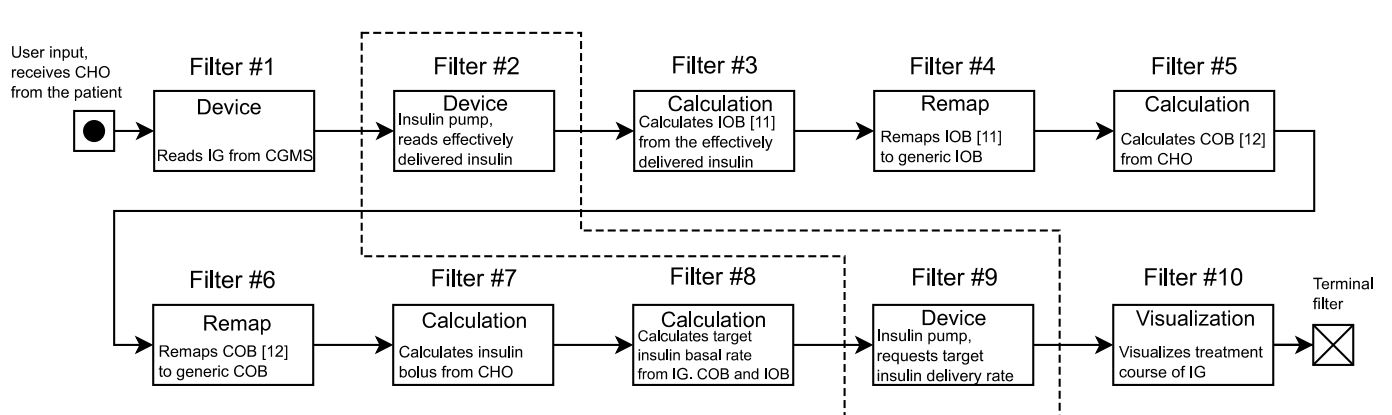
\includegraphics[width=1\textwidth]{img/scgms/filters.jpg}
\textit{Zdroj: SmartCGMS as an Environment for an Insulin-Pump  Development with FDA-Accepted In-Silico Pre-Clinical Trials \citep{cgms.ubl}}
\end{figure}

\textbf{Model} umožňuje načtení více hodnot voláním metody \textit{Get\_Continuous\_Levels} a jejich následné zpracování dle nastavených parametrů. Na rozdíl od filtru model zpracovává události dávkově. Je tak vhodný pokud potřebujeme pracovat s více signály najednou nebo predikovat hodnotu do budoucna. SmartCGMS obsahuje modely dynamiky glukózy Bergmanův model vylepšený Hovorkovo modelem a Koutného difúzním modelem, SimGlucose, s vynulovaným parametrem xi u UVA/Padova S2013, T1DMS a DMMS.R \citep{cgms.web}. Výpočet modelu je spušten filtrem \textit{Signal Generator} nebo filtrem \textit{Calculated Signal} pokud chceme  parametry modelu dynamicky spočítat pomocí solveru.

\textbf{Metrika} je druh filtru, který umožňuje spočítat metriky jako je například střední chyba, směrodatná odchylka nebo plocha pod křivkou \citep{cgms.koutny}.

Pro určení parametrů modelu lze využít \textbf{solver}. Ten na základě metrik signálů modelu spočítá jeho optimální parametry. Příkladem solveru je Meta-differential evolution, Pathfinder, Sequential brute force scan, Particle swarm optimization, Spiral optimization a další.

Vytvořené filtry, modely a solvery se zkompilují jako dynamické knihovna, která se načte při spuštění SmartCGMS. Aplikace také umožňuje integraci skriptů v jazyce Matlab. Skripty je nutné definovat v souboru \textit{matlab\_manifest.xml}.

SmartCGMS lze spustit v příkazové řádce (\textit{console3.exe}) nebo v grafickém uživatelském rozhraní (\textit{gpredict3.exe}). V záložce \textit{Filters} si uživatel nastaví jednotlivé filtry a jejich parametry. V záložce \textit{Simulation} pak spustí běh programu a může prohlížet grafy a logy s výstupy (příklad grafického výstupu je na obrázku \ref{fig:scgms_graf}). Konfiguraci lze uložit a poté opětovně načíst.

\begin{figure}[H]
\caption{Příklad výstupu SmartCGMS}
\label{fig:scgms_graf}
\centering
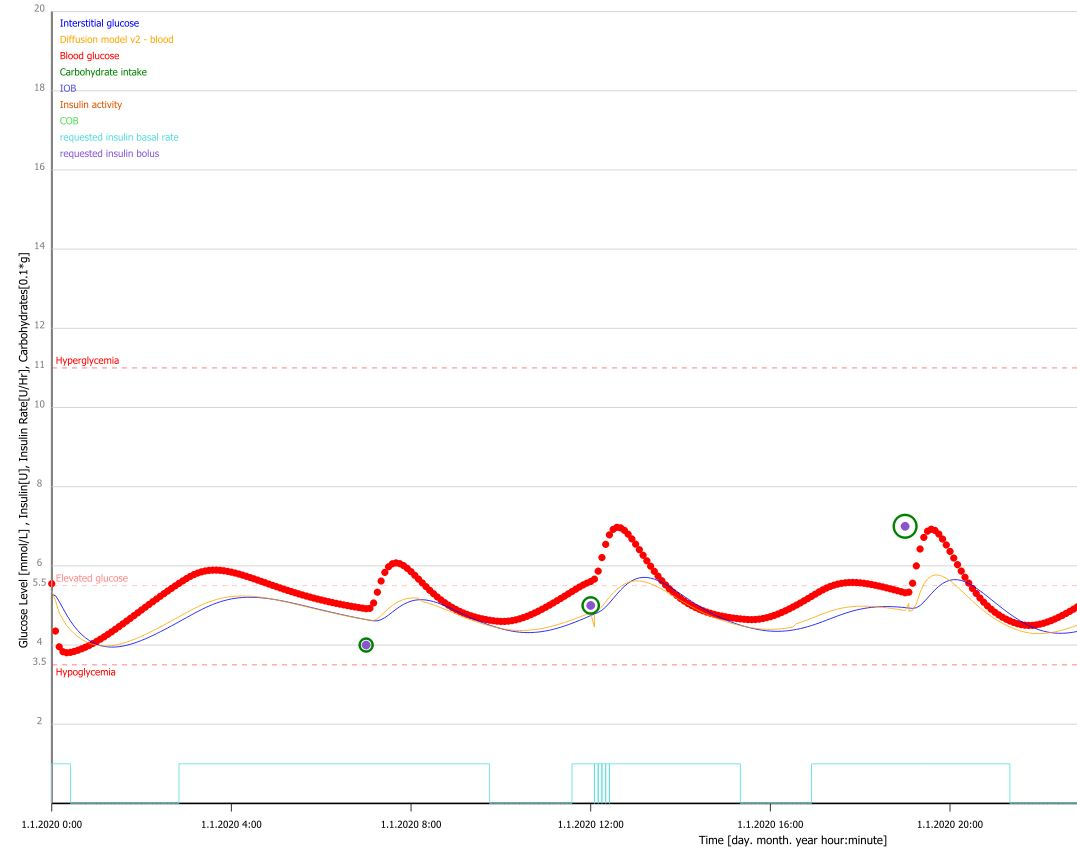
\includegraphics[width=1\textwidth]{img/scgms/graf1.jpg}
\textit{Zdroj: SmartCGMS}
\end{figure}

SmartCGMS je dostupný na \url{https://diabetes.zcu.cz/smartcgms}.
\chapter{Detekce příjmu karbohydrátů}

Pro detekci příjmu karbohydrátů jsem měl k dispozici anonymizovaná data ze senzoru CGMS. Data obsahují naměřené a zadané hodnoty:
\begin{itemize}
\setlength\itemsep{0em}
\item Glukóza v krvi (BG)
\item Intersticiální glukóza (IST)
\item Bazální množství inzulinu
\item Bolus inzulinu
\item Příjem karbohydrátů (CHO)
\item Fyzická aktivita
\item Kvalita spánku
\item Počet kroků
\item Srdeční tep
\item Vodivost kůže
\item Teplota kůže
\item Teplota okolí
\end{itemize}

Pro detekci karbohydrátů jsem implementoval tyto 3 metody:
\begin{itemize}
\setlength\itemsep{0em}
\item Long short-term memory neuronová síť (kapitola \ref{ch:lstm})
\item Lineární a kvadratická diskriminační analýza (kapitola \ref{ch:lda_qda})
\item Detekce hran pomocí thresholdů 1. diference hodnot intersticiální glukózy \\(kapitola \ref{ch:threshold})
\end{itemize}

Programovací jazyk pro zpracování dat ze senzoru, návrh a vyhodnocení jednotlivých metod jsem zvolil Python. Python jsem zvolil pro jeho knihovny NumPy, pandas a SciPy pro zpracování a analýzu dat, matplotlib pro vykreslení dat a knihovny TensorFlow a Keras pro práci s neuronovými sítěmi. Přestože je Python interpretovaný jazyk a tudíž pomalý při zpracování velkého množství dat, tyto knihovny jsou implementovány v jazyce C a optimalizovány pro vysoký výkon. Doba zpracování dat je tak srovnatelná s kompilovanými jazyky.

Implementace do SmartCGMS je v jazyce C++.

\section{Příprava dat}

CGMS senzor posílá data ve formě signálů, které mají strukturu:
\begin{itemize}
\setlength\itemsep{0em}
\item Logical Clock
\item Device Time
\item Event Code
\item Signal
\item Info
\item Segment Id
\item Event Code Id
\item Device Id
\item Signal Id
\end{itemize}

Příklad signálů ze senzoru CGMS je v tabulce \ref{tab:cgms_data}

\begin{table}[H]
\caption{Signály ze CGMS}
\label{tab:cgms_data}
\centering
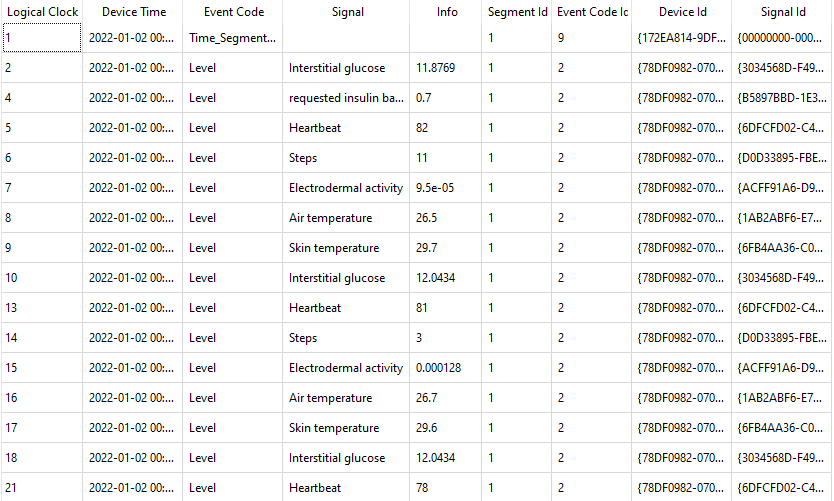
\includegraphics[width=1\textwidth]{img/cho/cgms_data.png}
\end{table}

Informaci pro následnou detekci v sobě nesou sloupce Device Time (čas měření), Signal (typ signálu) a Info (hodnota). Ty jsem extrahoval do dvourozměrné tabulky, kde řádky jsou čas měření a sloupce jednotlivé typy signálů.
Data intersticiální glukózy jsem interpoloval Akima spline \citep{cho.akima}, z níž jsem získal chybějící hodnoty a derivace 1. 2. a 3. řádu. Pro vyhlazení hodnot intersticiální glukózy jsem použil Savitzky-Golay filtr \citep{cho.savgol} řádu 3 s velikostí okna 21. Jelikož různé typy signálu nejsou měřeny ve stejný okamžik, řádky jsem seskupil podle sloupce intersticiální glukózy, která je měřena v pětiminutových intervalech.

V grafech na obrázku \ref{fig:48h_dataset} jsou transformovaná data naměřená senzorem CGMS za 48 hodin. Na prvním grafu jsou hodnoty Intersticiální glukózy a její vyhlazení Savitzky-Golay filtrem. Druhý graf znázorňuje zadanou bazální dávku inzulinu, bolusy, příjem karbohydrátů a fyzickou aktivitu. Na posledním grafu jsou zbylé měřené hodnoty.

\begin{figure}[H]
\caption{Data ze CGMS}
\label{fig:48h_dataset}
\centering
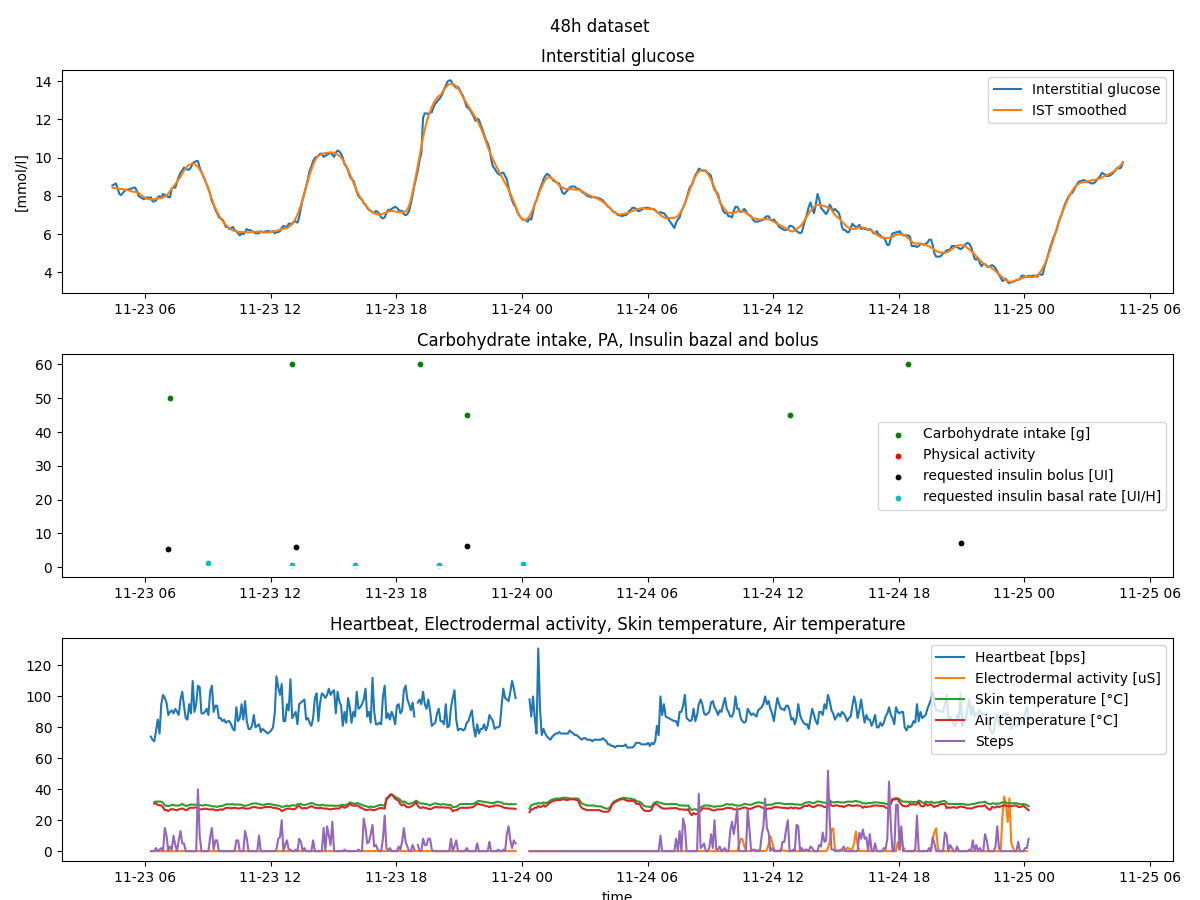
\includegraphics[width=1\textwidth]{img/cho/48h_dataset.png}
\end{figure}

\subsubsection{Spuštění}
Script pro transponaci dat se spustí zavoláním funkce:
\begin{verbatim}
load_log(patientID)
\end{verbatim}
ze souboru \texttt{load\_log.py}, kdy \textit{patientID} je ID pacienta. Logy musí být umístěny v adresáři data/. Pro spuštění transponace dat z více logů se zavolá funkce:
\begin{verbatim}
load_log_all(patientIDs)
\end{verbatim}
kdy \textit{patientIDs} je pole ID logů, které chceme transponovat. Transponovaná data jsou uložena do .csv souboru \textit{patientID-transposed.csv}.

Načtení a modifikace transponovaných dat se spustí voláním:
\begin{verbatim}
load_data(patientID, from_file, fill_missing, smooth,
           derivation, norm, verbose, graphs, analyze)
\end{verbatim}
ze souboru \texttt{load\_data.py}, potažmo
\begin{verbatim}
load_data_all(patientIDs, from_file, fill_missing, smooth,
                derivation, norm, verbose, graphs, analyze)
\end{verbatim}
pro načtení několika souborů. \textit{PatientID} je ID pacienta, \textit{from\_file} určuje zda se načtou již modifikovaná data nebo se spustí úprava transponovaných dat z logu. Parametr \textit{fill\_missing} určuje zda se mají nahradit chybějící hodnoty měření (\texttt{''} nenahrazuje se, 'akima' pro interpolaci Akima spline nebo 'mean' pro průměrnou hodnotu). Parametr \textit{smooth} určuje způsob filtrace ('savgol' pro Savitzky-Golay filter). Parametr \textit{derivation} určuje způsob výpočtu derivací ('akima' pro derivace Akima spline, 'gradient' pro numpy gradient, 'manual' pro výpočet diference). Parametr \textit{norm} říká, zda chceme data normalizovat ('std' normalizace směrodatnou odchylkou na interval <-1;1>, 'minmax' standardizace rozpětím na interval <0;1>). Parametr \textit{verbose} je pro vypsání průběhu zpracování dat, \textit{graph} zobrazí modifikovaná data v grafech a \textit{analyze} spustí analýzu dat z knihovny \textit{sweetviz}. Modifikovaná data jsou uložena do .csv souboru \textit{patientID-modified.csv}.


\section{Rekurentní neuronové sítě}
\label{ch:lstm}

Rekurentní neuronové sítě jsou vhodné pro predikci sekvenčních dat (například časové řady). Vyznačují se tím, že si předávají informaci o předchozím stavu (aktivaci skryté vrstvy):

$H_{t}=\sigma (W_{h}H_{t-1}+W_{x}X_{t}+b)$

\noindent kde $W$ jsou váhy a $b$ je bias. Neurony, které takto uchovávají svůj stav, se nazývají buňky. Riziko RNN spočívá v náchylnosti vzniku jevu označovaného jako mizející nebo explodující gradient vznikajícího při zpětné propagaci, kdy hodnoty exponenciálně klesají nebo rostou. To je z důvodu, že se chyba propaguje přes všechny iterace. Tento problém eliminuje long short-term memory nebo gated recurrent unit neuronová síť.

\begin{figure}[H]
\caption{Rekurentní neuronová síť}
\label{fig:rnn}
\centering
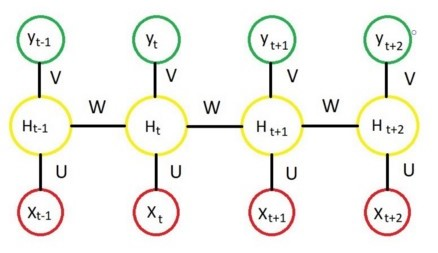
\includegraphics[width=0.7\textwidth]{img/cho/rnn.jpeg}\\
\textit{Zdroj: https://medium.com/}
\end{figure}

\subsection{Long short-term memory}

Long short-term memory neuronová síť (LSTM) je speciální případ rekurentní neuronové sítě. V každé iteraci si buňka uchovává dodatečnou informaci nazvanou \textit{memory}. 

Nejprve se ze vstupního vektoru $X_{t}$ a stavu předchozí buňky $H_{t-1}$ spočte Forget gate $f_{t}$, Candidate layer $\bar{C}_{t}$ Input gate $I_{t}$ a Output gate $O_{t}$ \citep{cho.lstm}:

$f_{t}=\sigma(X_{t} \otimes U_{f}+H_{t-1} \otimes W_{f})$\\\indent
$\bar{C}_{t}=tanh(X_{t} \otimes U_{c}+H_{t-1} \otimes W_{c})$\\\indent
$I_{t}=\sigma(X_{t} \otimes U_{i}+H_{t-1} \otimes W_{i})$\\\indent
$O_{t}=\sigma(X_{t} \otimes U_{u}+H_{t-1} \otimes W_{u})$

\noindent kde $W$ a $U$ jsou váhové vektory. Následně se spočte \textit{memory} prvek $C_{t}$:

$C_{t}=f_{t} \otimes C_{t-1} \oplus I_{t} \otimes \bar{C}_{t}$

\noindent a výstupní stav $H_{t}$:

$H_{t}=O_{t} \otimes tanh(C_{t})$

Diagram LSTM buňky je na obrázku \ref{fig:lstm_cell}.

\begin{figure}[H]
\caption{LSTM buňka}
\label{fig:lstm_cell}
\centering
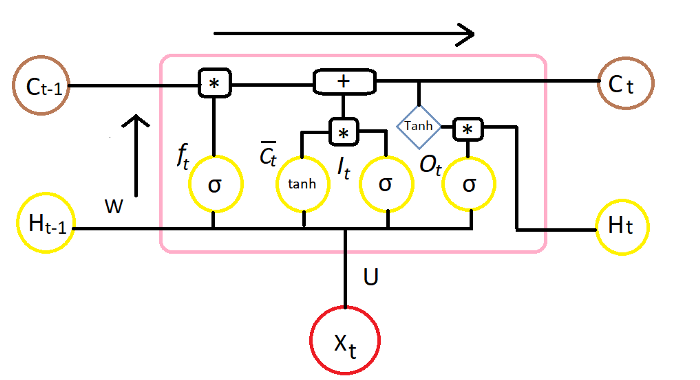
\includegraphics[width=1\textwidth]{img/cho/lstm_cell.png}
\textit{Zdroj: https://medium.com/}
\end{figure}

\subsection{Gated recurrent unit}

Gated recurrent unit neuronová síť (GRU) využívá Update gate $z_{t}$ a Reset gate $r_{t}$. Ty určují která informace bude propagována na výstup. Mohou tak vytěžit relevantní informace. Update a reset gate se spočte \citep{cho.gru}:

$z_{t}=\sigma(W_{z}x_{t} + U_{z}h_{t-1})$\\\indent
$r_{t}=\sigma(W_{r}x_{t} + U_{r}h_{t-1})$

\noindent kde $W$ a $U$ jsou váhové vektory. Následně se spočte relevantí informace z předchozího stavu $\bar{h}_{t}$:

$\bar{h}_{t}=tanh(W_{h}x_{t} + U_{h}(r_{t} \otimes h_{t-1}))$

\noindent a výstupní stav $h_{t}$:

$h_{t}=z_{t} \otimes h_{t-1} + (1-z_{t}) \otimes \bar{h}_{t}$

Diagram GRU buňky je na obrázku \ref{fig:gru_cell}.

\begin{figure}[H]
\caption{GRU buňka}
\label{fig:gru_cell}
\centering
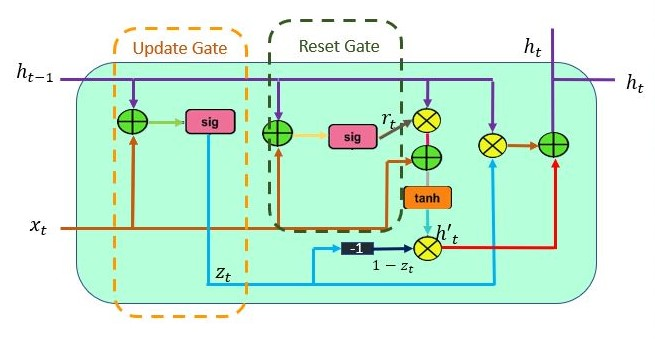
\includegraphics[width=1\textwidth]{img/cho/gru_cell.jpg}
\textit{Zdroj: https://www.pluralsight.com/}
\end{figure}

\subsection{Model}

Pro detekci karbohydrátů jsem sestavil sekvenční keras\footnote{Keras je nadstavba nad knihovnou TensorFlow pro neuronové sítě} model se čtyřmi vrstvami:
\begin{itemize}
\setlength\itemsep{0em}
\item Obousměrná LSTM nebo GRU
\item Dropout(0,5)
\item Dense(128)
\item Dense(1)
\end{itemize}

První vrstvou je rekurentní neuronová síť. Ta může být buď LSTM nebo GRU. Tato vrstva má 128 neuronů a dropout 0,2. Vstupem vrstvy je časové okno N vstupních prvků velikosti W. Tvar vstupních dat je WxN:

$\begin{bmatrix}
X^{1}_{1} & X^{2}_{1} & ... & X^{N}_{1}\\
X^{1}_{2} & X^{2}_{2} & ... & X^{N}_{2}\\
... & ... & ... & ...\\
X^{1}_{W} & X^{2}_{W} & ... & X^{N}_{W}
\end{bmatrix}$

Dropout vrstva s \textit{rate=0,2} náhodně nastaví některé vstupy na nulu v poměru 0,2. Nevynulované vstupy jsou škálovány 1/(1-rate), takže součet všech vstupů je nezměněn. To zabrání přetrénování neuronové sítě. Droupout vrstva je aplikována pouze při trénování sítě. První Dense vrstva (propojení neuronů formou každý s každým) má 128 neuronů, aktivační funkce je \textit{relu}. Druhá Dense vrstva s jedním neuronem je výstupní.

Jako ztrátová funkce je použita střední kvadratická chyba (MeanSquaredError), optimalizační algoritmus je Adam. Z datasetu je 80 \% dat použito pro trénování a 20 \% pro validaci. Data jsou do neuronové sítě dávkována v dávkách o velikosti 64. Jelikož se jedná o časovou řadu, data se nepromíchávají.

\subsubsection{Spuštění}

Trénování neuronové sítě se spustí voláním funkce:
\begin{verbatim}
lstm(df, headers, label, type, width, epochs)
\end{verbatim}
ze souboru \texttt{cho\_detection.py}, kde \textit{df} je pandas dataframe modifikovaných dat, \textit{headers} je pole názvů sloupců vstupních dat, \textit{label} je predikovaná třída, \textit{type} je LSTM nebo GRU, \textit{width} je velikost okna a \textit{epochs} je počet epoch, kolikrát má proběhnout trénovací cyklus.

Natrénovaný model se uloží do souboru \texttt{model/[patientID]\_keras\_model.h5} a následně se exportuje do souboru \texttt{model/[patientID]\_fdeep\_model.h5}, který používá C++ knihovna frugally-deep (viz kapitola \ref{ch:implementace_scgms}).

\subsubsection{Výsledky}

Pro detekci karbohydrátů jsem jako vstupní prvky zvolil vyhlazená data intersticiální glukózy, jejich derivaci 1. řádu a minuty normalizované na interval <0;1>. Velikost okna je 24 (tj. 2 hodiny). Predikovaná třída je množství zadaných karbohydrátů. Tyto hodnoty jsou pro účel trénování rozkopírovány po dobu dvou hodin od času zadání. Neuronová síť je trénovaná ve 200 epochách.

Výstupem jsou predikované odhady karbohydrátů. Pro detekci příjmu karbohydrátů určíme threshold. Pakliže množství karbohydrátů predikovaných neuronovou sítí je větší než tento threshold, je detekováno jídlo. Threshold je pro každého pacienta jiný.

\textbf{//TODO}

\section{Lineární a kvadratická diskriminační analýza}
\label{ch:lda_qda}

Diskriminační analýzu jsem se rozhodl implementovat vzhledem k vysoké úspěšnosti a malému zpoždění, které dosáhli \citet{Analyza.LDA} v článku \textbf{Pattern Recognition Reveals Characteristic Postprandial Glucose Changes: Non-Individualized Meal Detection in Diabetes Mellitus Type 1} (kapitola \ref{ch:lda}).

\subsection{Teorie}
Diskriminační analýza slouží k rozdělení prvků do konečného počtu tříd na základě lineární kombinace charakteristických prvků. Pro klasifikaci potřebujeme znát posteriory tříd \textbf{P(Y|X)}. Pravděpodobnostní model \textbf{P(X|y=k)} pro každou třídu \textbf{k} lineární a kvadratické diskriminační analýzy je dán vícerozměrnou Gaussovo distribucí \citep{cho.book.lda}:

\scalebox{1.2}{$P(X|y=k)=\frac{1}{(2\pi)^{p/2}|\sum_{k}|^{\frac{1}{2}}}e^{-\frac{1}{2}(x-\mu_{k})^{T}\sum^{-1}_{k}(x-\mu _{k})}$}\\\\
kde \textbf{p} je počet prvků. Pro predikci je pak použito Bayesovo rozhodovací pravidlo \citep{cho.book.lda}:

\scalebox{1.2}{$P(y=k|x)=\frac{P(x|y=k)P(y=k)}{P(x)}=\frac{P(x|y=k)P(y=k)}{\sum_{l}{P(x|y=l)P(y=l)}}$}\\\\
kdy hledáme třídu s maximálním posteriorem.

Logaritmus posterioru pro kvadratickou diskriminační analýzu (QDA) je \citep{cho.book.lda}:

$P(y=k|x)=-\frac{1}{2}log|\sum_{k}|-\frac{1}{2}(x-\mu_{k})^{T}\sum^{-1}_{k}(x-\mu_{k})+logP(y=k)$\\\\
Predikovaná třída je ta, která má maximální logaritmický posterior.

Lineární diskriminační analýza (LDA) je speciální případ QDA, kdy předpokládáme, že třídy mají stejnou kovarianční matici. Logaritmus posterioru je pak vyjádřen \citep{cho.scikit.lda}:

$P(y=k|x)=-\frac{1}{2}(x-\mu_{k})^{T}\sum^{-1}(x-\mu_{k})+logP(y=k)$\\

Vstupem diskriminační analýzy může být buď množina prvků pro daný časový okamžik nebo časové okno jednoho prvku. Predikované třídy jsou příjem/nepříjem karbohydrátů. Ty dostaneme převedením sloupce karbohydrátů na booleanovskou proměnnou (0 je false, cokoli větší než 0 je true).

\subsection{Množina prvků}

Nejčastějším vstupem diskriminační analýzy je množina charakteristických prvků $X_{i}$. V tomto případě se diskriminační analýza snaží rozdělit prostor tak, aby odlišila jednotlivé třídy (viz obrázek \ref{fig:lda}).

\begin{figure}[H]
\caption{Rozdělení prostoru lineární diskriminační analýzou dvou prvků}
\label{fig:lda}
\centering
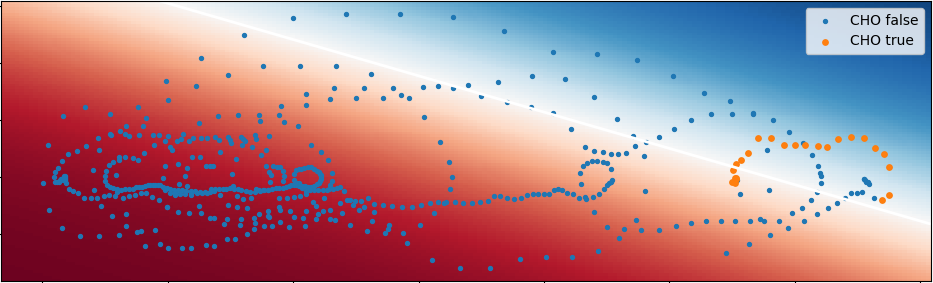
\includegraphics[width=1\textwidth]{img/cho/lda2.png}
\end{figure}

\subsubsection{Spuštění}

Trénování LDA a QDA pro množinu prvků se spustí voláním funkce:
\begin{verbatim}
lda(df, headers)
\end{verbatim}
ze souboru \texttt{cho\_detection.py}, kde \textit{df} je pandas dataframe modifikovaných dat, \textit{headers} je pole názvu sloupců vstupních dat.

\subsubsection{Výsledky}

\textbf{//TODO}

\subsection{Časové okno}

V případě časového okna muže být na vstupu pouze jediný prvek. To je dáno tím, že vstupem diskriminační analýzy je jedno-dimenzionální pole dat. Vstupní data mají tvar:

$\begin{bmatrix}
X_{i-W} & X_{i-W-1} & ... & X_{i-1} & X_{i}
\end{bmatrix}$

\noindent kde W je velikost časového okna.

\subsubsection{Spuštění}

Trénování LDA a QDA pro časové okno se spustí voláním funkce:
\begin{verbatim}
lda_window(df, header, width)
\end{verbatim}
ze souboru \texttt{cho\_detection.py}, kde \textit{df} je pandas dataframe modifikovaných dat, \textit{header} je název sloupce vstupních dat a \textit{width} je velikost okna.

\subsubsection{Výsledky}

\textbf{//TODO}


\section{Detekce hran průběhu intersticiální glukózy}
\label{ch:threshold}

Tato metoda detekuje vzestupné a klesající hrany průběhu intersticiální glukózy pomocí thresholdů první diference měřených hodnot intersticiální glukózy.

Derivace funkce $f'(x)$ v bodě $x$ je směrnicí tečny funkce $f(x)$ v daném bodě. Pakliže je funkce $f(x)$ v bodě $x$ rostoucí, je její směrnice tečny v bodě $x$ kladná. Pokud je $f(x)$ klesající, její směrnice tečny je v daném místě záporná. Velikost derivace v bodě $x$ pak udává velikost změny $f(x)$, neboli říká, jak strmě funkce stoupá či klesá. Derivace funkce $f(x)$ v bodě $x_{1}$ můžeme vyjádřit jako:

\scalebox{1.2}{$f'(x) = \frac{d}{dx}f(x) = \lim_{x \to x_{0}} \frac{f(x)-f(x_{0})}{x-x_{0}}$}

Jelikož data ze senzoru CGMS jsou diskrétní, můžeme derivaci nahradit rovnicí první diference. Pro data intersticiální glukózy tak dostáváme vztah:

\scalebox{1.2}{$\Delta IST = \frac{IST_{t} - IST_{t-1}}{\Delta t}$}

Naměřená data intersticiální glukózy mohou být zatížena šumem a případně i dočasnými výchylkami hodnot glukózy. Každá taková výchylka pak má značný vliv na hodnotu derivace. Z toho důvodu je potřeba data před výpočtem vyhladit. Pro vyhlazení dat jsem zvolil digitální Savitzky-Golay filtr. Každá podmnožina $2m+1$ prvků je vzorkována na polynom stupně $p (p\leq 2m)$ ve smyslu nejmenších čtverců \citep{cho.savgol}. Zvolil jsem polynom stupně 3 a velikost podmnožiny 21. Vyhlazená data vidíme v grafu na obrázku \ref{fig:savgol}.

\begin{figure}[H]
\caption{Vyhlazená data intersticiální glukózy}
\label{fig:savgol}
\centering
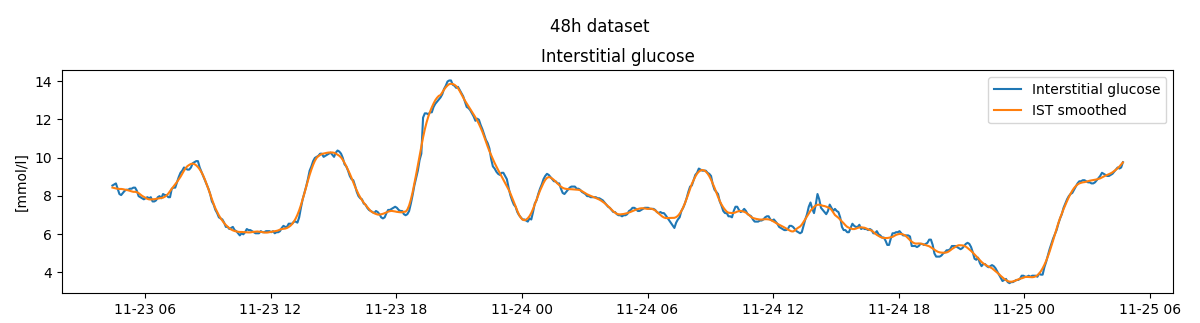
\includegraphics[width=1\textwidth]{img/cho/savgol.png}
\end{figure}

Následně se data ohodnotí. Pokud $\Delta IST$ překročí určitý threshold $th_{i}$, přiřadí se váha $w_{i}$. Takových dvojic thresholdů a vah může být libovolné množství. Experimentálně byla zjištěna kombinace thresholdů $th=[0.0125, 0.018]$ a vah $w=[2.25, 3]$.

Samotné ohodnocení podle thresholdů zachytí jakýkoli jednorázový větší výkyv v datech intersticiální glukózy. Jelikož příjem karbohydrátů se projevuje zvýšením glykémie v řádu desítek minut až hodin, chceme znát vývoj křivky intersticiální glukózy v čase. Z toho důvodu pro kladně ohodnocená data zvýšíme ohodnocení v případě, že předchozí hodnoty vykazují vzrůstající trend po dobu dvou hodin nazpět (tj. 24 hodnot, data jsou vzorkována po pěti minutách). Získáme tak aktivační funkci pro rostoucí hrany.
\begin{verbatim}
if activation[i] > 2:
  for j in range(24):
    if activation[i-j] >= 2+0.2*j:
      activation[i] += 0.1*j
\end{verbatim}
Pro klesající hrany použijeme stejný postup, ale se záporným ohodnocením.

\subsubsection{Spuštění}

Detekce hran průběhu intersticiální glukózy se spustí voláním funkce:
\begin{verbatim}
threshold(df, th, weight)
\end{verbatim}
ze souboru \texttt{cho\_detection.py}, kde \textit{df} je pandas dataframe modifikovaných dat (load\_data musí být spuštěno s parametry smooth='savgol', derivation='difference', norm=''), \textit{th} je pole thresholdů a \textit{weight} je pole vah o stejné délce. Funkce vrací hodnoty aktivační funkce.

\subsubsection{Výsledky}
V grafu na obrázku \ref{fig:hrany} je ukázka detekce hran. Červeně je aktivace vzestupné hrany, modře aktivace sestupné hrany posunuté. Počátek sestupné hrany je posunut na úrověň poslední hodnoty aktivace vzestupné hrany. Mezi vzestupnou a sestupnou hranou je vždy několik hodnot, kdy byla hladina intersticiální glukózy vyrovnaná.

\begin{figure}[H]
\caption{Detekované hrany průběhu intersticiální glukózy}
\label{fig:hrany}
\centering
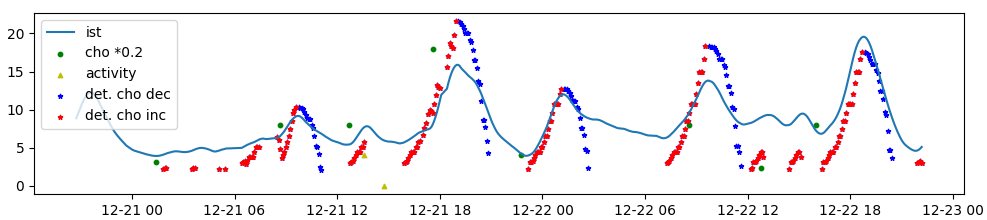
\includegraphics[width=1\textwidth]{img/cho/hrany.png}
\end{figure}

Jídlo je detekováno, pakliže aktivační funkce vzestupné hrany je větší než zvolený threshold. Nízký threshold detekuje většinu jídel, ale také může detekovat výkyvy nesouvisející s příjmem karbohydrátů. Naopak vysoce zvolený threshold nebude detekovat menší jídla. Řešením je použití více thresholdů pro stanovení pravděpodobnosti jídla.

\textbf{//TODO}

%Výsoký počet falešně pozitivních výsledků se mi částečně podařilo redukovat při implementaci do SmartCGMS.


\section{Implementace do SmartCGMS}
\label{ch:implementace_scgms}

Do SmartCGMS jsem implementoval filtr pro detekci karbohydrátů pomocí detekce hran průběhu intersticiální glukózy a pomocí rekurentních neuronových sítí. Dále bylo potřeba implementoval Savitzky-Golay filtr pro vyhlazení dat a evaluační filtr. Vytvořené filtry jsou zkompilovány do knihovny \texttt{cho\_detection.dll}.

Filtry implementují rozhraní \textit{scgms::IFilter} a \textit{refcnt::IReferenced}. Při vytvoření instance filtru se volá metoda \textit{Configure}, která slouží pro nastavení filtru (typicky přečtení a nastavení konfiguračních parametrů). Metoda \textit{Execute} je volána pokaždé, když přijde signál od předchozího filtru. Tato metoda vykonává požadovanou funkcionalitu. Původní událost se na závěr zpravidla posílá dalšímu filtru. Současně se musí zaregistrovat descriptor nového filtru, který definuje ID filtru, název a konfigurační parametry, a případně i descriptor nového signálu. Vytvořená dynamická knihovna musí exportovat funkce \textit{do\_create\_filter}, \textit{do\_get\_filter\_descriptors} a \textit{do\_get\_signal\_descriptors}.

Data mohou být rozdělena do časových segmentů dle měření. V takovém případě filtry pracují s každým segmentem zvlášť. Rozdělení do segmentů je realizováno pomocí mapy, kdy klíčem je ID segmentu.

Implementované algoritmy pracují s daty v určitém časovém okně. Pro tyto účely jsem vytvořil vlastní spojový seznam na principu klouzavého okénka \textbf{swl}. Ten dědí od \textit{std::deque}, které umožňuje vkládání prvků z obou stran i indexaci. konstruktor má jeden parametr určující velikost okna. Při vložení nadlimitního prvků se odebere prvek z druhého konce seznamu.

\textbf{Savitzky-Golay} filtr počítá vyhlazená data intersticiální glukózy. Výstupem je \textbf{IST smoothed} signál.

\textbf{CHO detection} filtr počítá aktivační funkci a detekci karbohydrátů. To je implementováno rekurentní neuronovou sítí nebo detekcí hran průběhu intersticiální glukózy. Filtr posílá dva signály. \textbf{Activation} signál je výstup použitého algoritmu a \textbf{CHO probability} udávající detekovaný příjem (1 - nižší pravděpodobnost, 2 - vyšší pravděpodobnost).

Rekurentní neuronová síť využívá natrénovaného keras modelu. Ten je možné použít v C++ pomocí knihovny frugally-deep \citep{cho.frugally}. Model je nutné konvertovat pomocí skriptu \texttt{keras\_export/convert\_model.py}, který je součástí frugally-deep knihovny. Podporované sítě jsou LSTM i GRU. Příklad konfigurace s GRU je v konfiguračním souboru \texttt{setup\_gru.ini} (viz příloha B).
 
V případě detekce hran jsou nastaveny 2 thresholdy. Nižší pro brzkou detekci, která ale může detekovat výkyvy nesouvisející s příjmem jídla. Vyšší threshold je potvrzovací, kdy existuje vysoká pravděpodobnost příjmu karbohydrátů. Detekce je pouze pro vzestupnou hranu. Potvrzení může být i pomocí rekurentní neuronové sítě. Příklad konfigurace thresholdů je v konfiguračním souboru \texttt{setup\_th.ini} (viz příloha B).

\textbf{Evaluate} filtr vyhodnocuje úspěšnost detekce. Pravdivě pozitivní (TP) jsou hodnoty, kdy je jídlo detekováno (hodnota detekce alespoň 1) do dvou hodin od jeho zadání pacientem. Pokud je hodnota detekce 2, je jídlo bráno jako potvrzeno. Pakliže jídlo není detekováno do dvou hodin od zadání, je výsledek falešně negativní (FN). V případě detekce hodnoty 2, kdy jídlo není zadané, výsledek je falešně pozitvní (FP). Zároveň je počítáno zpoždění detekce od zadání jídla pacientem. Jelikož v datech nemusí být některá jídla zadaná, statistika každého dne se započítá pouze tehdy, kdy byly zadány alespoň 3 jídla. Evaluate filtr neřeší časové segmenty.

\subsubsection{Výsledky}

Algoritmy byly testovány na datech jedenácti pacientů. Výsledky pro jednotlivé pacienty jsou v souboru \textit{results.txt}. V tabulce \ref{tab:results} jsou souhrnné výsledky.

\begin{table}[H]
\caption{Výsledky}
\label{tab:results}
\begin{tabular}{|l|c|c|c|}
\hline 
& \textbf{Detekce hran} & \textbf{Detekce hran (+GRU)} & \textbf{ GRU }\\
\hline 
\hline 
Jídel & 340 &  &  \\\hline
Úspěšnost & 85 \% &  &  \\\hline
TP & 289 &  &  \\\hline
TP/pacient & 26,27 &  &  \\\hline
TP potvrzeno & 167 &  &  \\\hline
Potvrzeno & 57,8 \% &  &  \\\hline
FN & 45 &  &  \\\hline
FN/pacient & 4,09 &  &  \\\hline
FP & 112 &  &  \\\hline
FP/pacient & 10,18 &  &  \\\hline
Zpoždění* & 27,54 &  &  \\
\hline
\end{tabular}
\begin{flushleft}
* průměrná doba detekce karbohydrátů od příjetí jídla v minutách\\
TP - true positive\\
FN - false negative\\
FP - false positive\\
\end{flushleft}
\end{table}

Průměrná úspěšnost detekce jídla je 85 \% s průměrným zpožděním 27,54 minut. Všechny algoritmy vykazují vysoký počet falešně pozitivních výsledků. To může být dáno častými výkyvy glukózy u pacienta nebo tím, že pacient jídlo nezadal, nebo ho zadal pozdě.

\bibliographystyle{csplainnatkiv}
{\raggedright\small
\bibliography{literatura}
}

%\chapter*{Příloha A: Tabulky}
\addcontentsline{toc}{chapter}{Příloha A: Tabulky}


\begin{figure}[H]
\caption{Data ze CGMS}
\label{tab:cgms_data}
\centering
\begin{sideways}
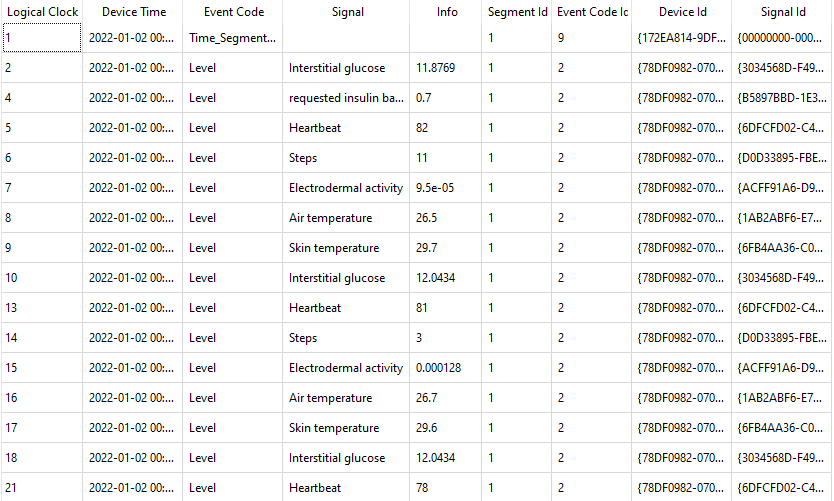
\includegraphics[height=0.28\textheight]{img/cho/cgms_data.png}
\end{sideways}
\end{figure}


\end{document}
